% Copyright (C) 2007 Thomas L. Kula
% All Rights Reserved
%
% See the file LICENSE for license terms.
\documentclass[12pt]{article}
\usepackage{graphicx}
\setlength{\paperwidth}{5.5in}
\setlength{\paperheight}{8.5in}
\setlength{\textheight}{7.45in}
\setlength{\topmargin}{-1.0in}
\setlength{\oddsidemargin}{-0.5in}
\setlength{\evensidemargin}{-0.5in}
\setlength{\textwidth}{4.0in}
\setlength{\parindent}{0in}
\setlength{\parskip}{3mm}
\usepackage[print]{booklet} \nofiles
\source{\magstep0}{5.5in}{8.5in}
\target{\magstep0}{11in}{8.5in}
\setpdftargetpages
\pagestyle{empty}
\begin{document}



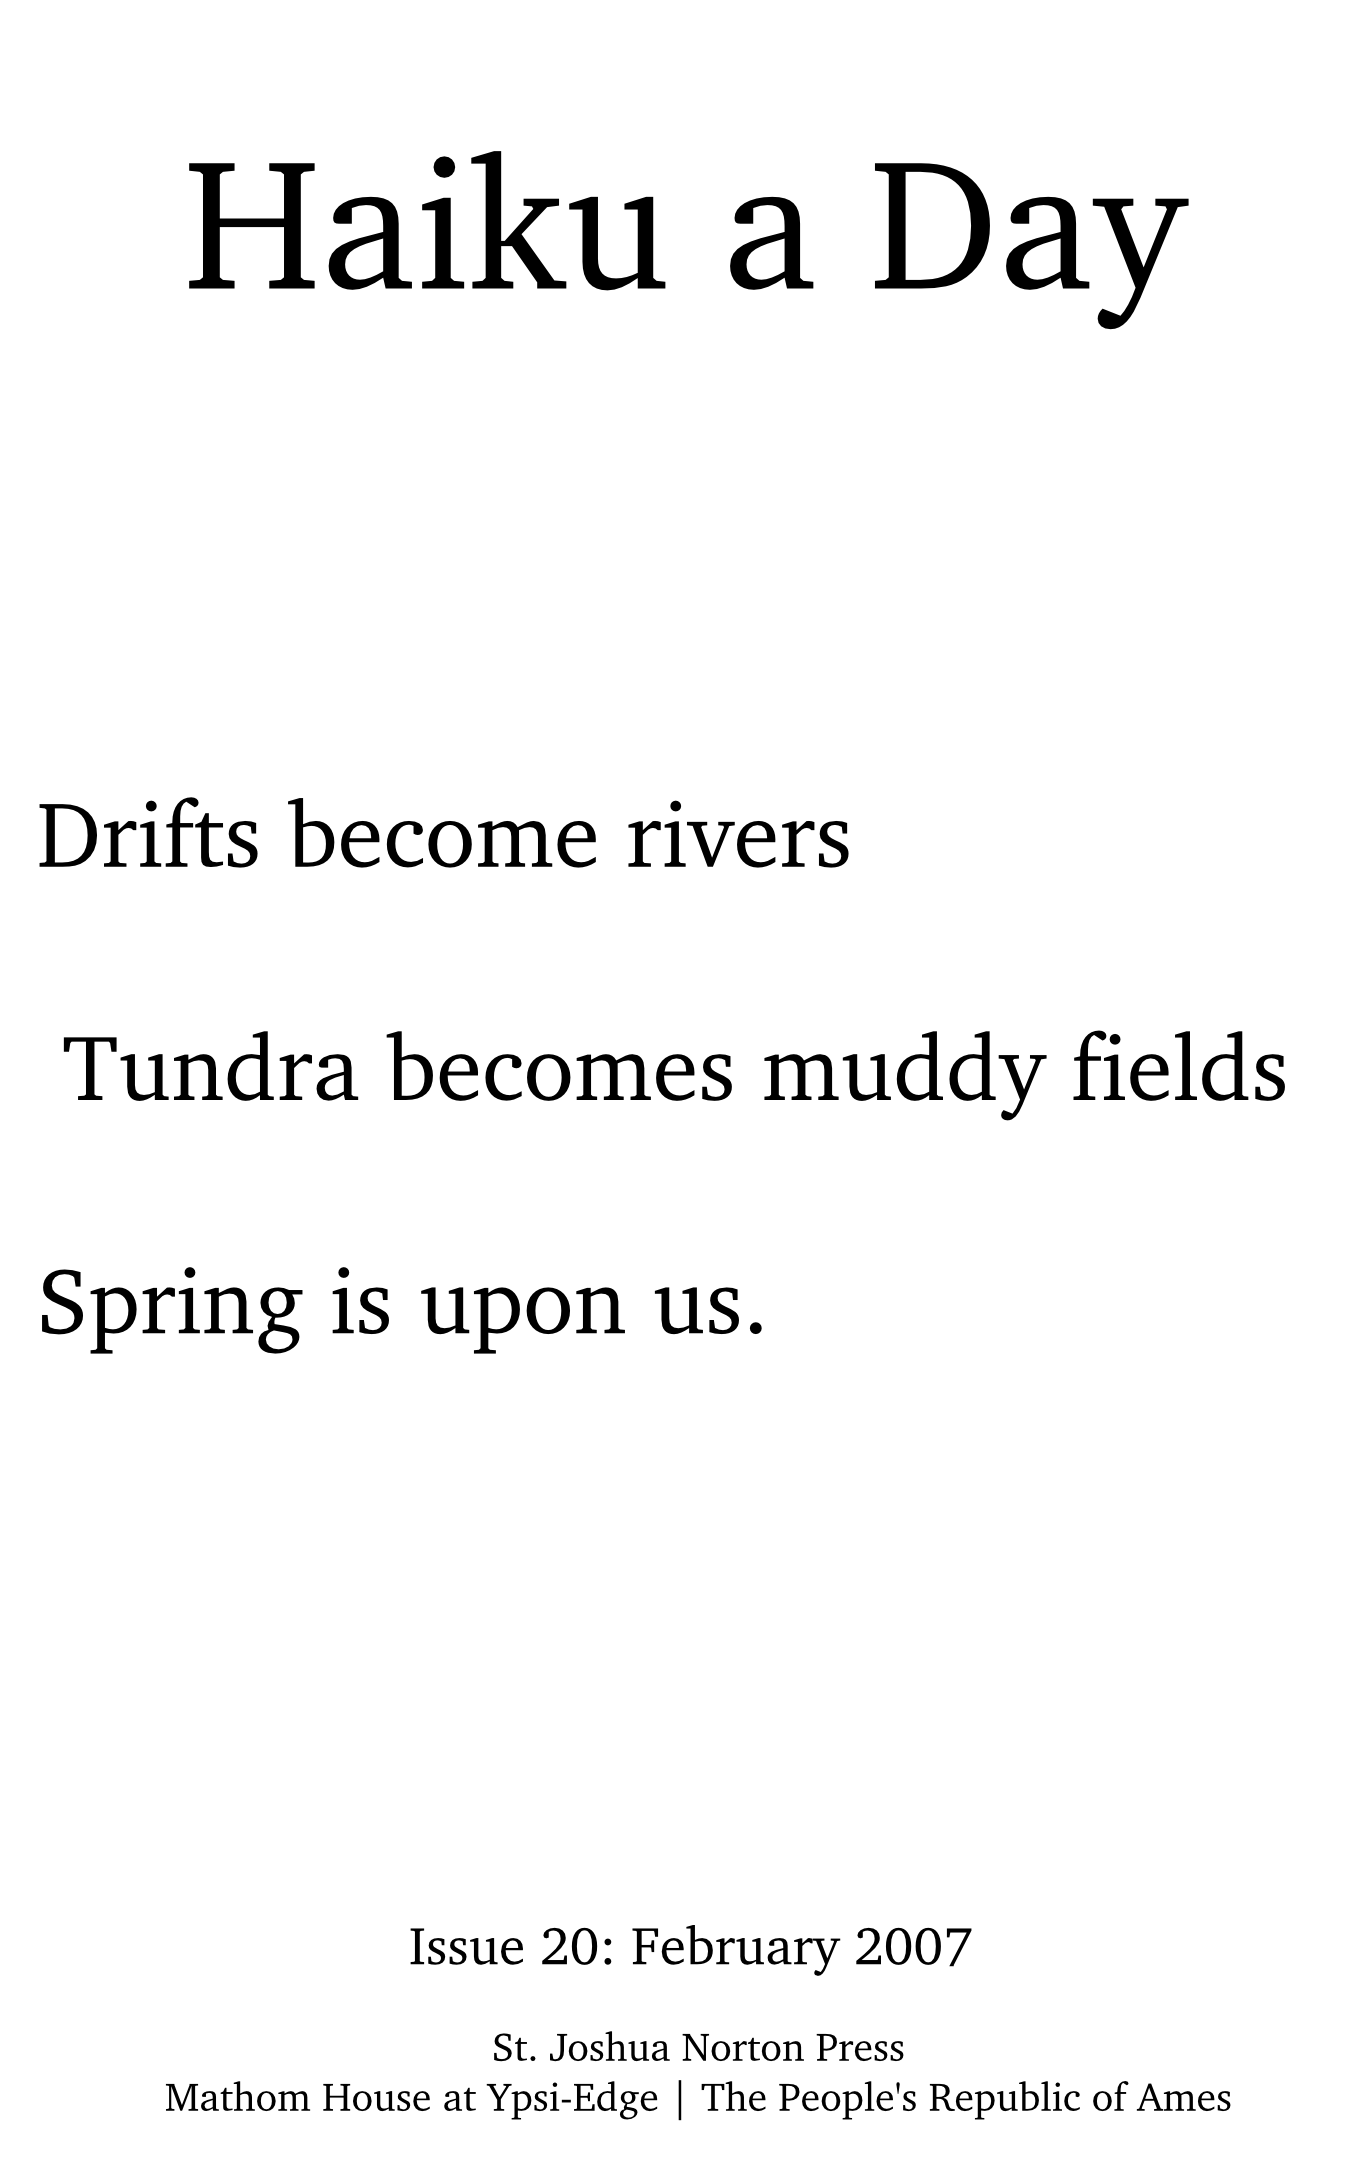
\includegraphics{frontpage.png}

\newpage

I am filled with hope today as the first glimmers
of spring poke their head out of the winter doldroms.
It was in the 50s here today, and the yards of 
Ypsilanti are flowing with the runoff of snow that
is quickly melting. Walking around, stopping at
the post office and picking up some things and
enjoying the weather put me in good spirits. 

--- Thomas

http://kula.tproa.net/had/ \\
kula@tproa.net

Download this and previous HADs at the website, so you can
print out you own (DIY, yeah!) or if you want me to send
you one, send me your address, and maybe a stamp if you
are feeling nice. Or send me something you've made ---
trades always appreciated.

1 February 2007  

Kitchen guardian \\
The gnome looks down from on high \\
Guarding my popcorn 

2 February 2007

Lines in the carpet \\
Fun with the vacuum cleaner \\
It does suck that much 

3 February 2007

The brisk wind blows bright \\
Clouds of snow across the ground; \\
The sun laughs up high. 

4 February 2007

Hey AATA \\
Why does the seven not go \\
Past me on Sundays? 

\newpage

5 February 2007

Hot water bottle \\
Keeping my wee toes toasty \\
Happiness cocoon 

6 February 2007

A good music store \\
Narrow aisles, pure chaos \\
Condensed paradise 

7 February 2007

In the Winter's gasp \\
The sigh of Spring can be heard \\
Low, breathy, distant. 

8 February 2007

Fiery, wirey snake \\
Glowing darkly in a pit \\
Barely tame fire 

9 February 2007

Late night search for food \\
Two places did betray us \\
The last one saved us 

10 February 2007

A thread pulls free \\
Escaping my sweater's grasp \\
Run free, little string! 

11 February 2007

Save us Rocket Dog! \\
Drive away the evil cats \\
Give the dog a bone 

\newpage

12 February 2007

Behold the closet! \\
Full of junk I should clean up \\
Close the door; ignore. 

13 February 2007

Box of dusty books \\
A piece of paper slips out \\
Old letter, once lost. 

14 February 2007

The French press broken \\
Shattered glass and tea leaves fall \\
Third one in a month 

15 February 2007

Malestrom of hot air \\
Glowing, spinning, dark red pit \\
From it comes popcorn 

16 February 2007

Mail flows to Paris \\
The French host is corrected \\
service-fr2 

17 February 2007

Toes frozen for peace \\
I search for new shoes in vain \\
Can order Monday 

18 February 2007

A cave of blankets \\
The cruel world outside my bed \\
I snug in for warmth. 

\newpage

19 February 2007

Rooibos brewing \\
And dinner is resting well \\
Reading beakons me. 

20 February 2007

The sun earlier \\
Breaks into the morning sky \\
Fuck I need some tea 

21 February 2007

The car, it won't start \\
Stray lights leave battery sad \\
Cripes, I hate driving 

22 February 2007

Two evening coffees \\
Disrupting the sleep patterns \\
Denying slumber 

23 February 2007

Behold the Cheese Plate! \\
Armadillo of crackers \\
Dinner most sublime 

24 February 2007

Map delineates \\
The paths on which I should bike  \\
Blazing across town

25 February 2007

A snowy drive out \\
Picking up a new bike frame \\
A good 10 bucks spent

\newpage

26 February 2007

Turn around record \\
Spinning about your axis \\
Groovy music grooves

27 February 2007

Time stops suddenly \\
The stars burst brightly before \\
Falling to madness

And with all credit due to the late great Johnny Cash:

28 February 2007

I hear the train come \\
Around the bend; Not seen sun \\
Since I don't know when.

Here in Folsom Town \\                                                                     
I am stuck in a prison \\
Time keeps draggin' on 
                                                                                                                          
That whistle blowing \\ 
I hear it, yea I hear it \\
Down to San Antone 
                                                                                                       
A baby was I \\
Mama said be a good boy \\
Do not play with guns 
                                                                                                                          
But there in Reno \\ 
I shot a man in cold blood \\
Just to watch him die  

Blow now that whistle \\
I hear it, hang my head down \\
I hang it and cry 

\newpage

In a fancy car  \\ 
Rich folks eat, and drink coffee \\
And smoke big cigars 
                                                                                                                          
I know this my fate \\
I can't be free, yet they move \\
That's what tortures me         
                                                                                                                          
If I could be free \\ 
If that railroad train was mine \\ 
I'd move down the line                                                                                                    
                                                                                                                          
From Folsom Prison \\
Far I would stay; that whistle \\
Blow my blues away

\newpage

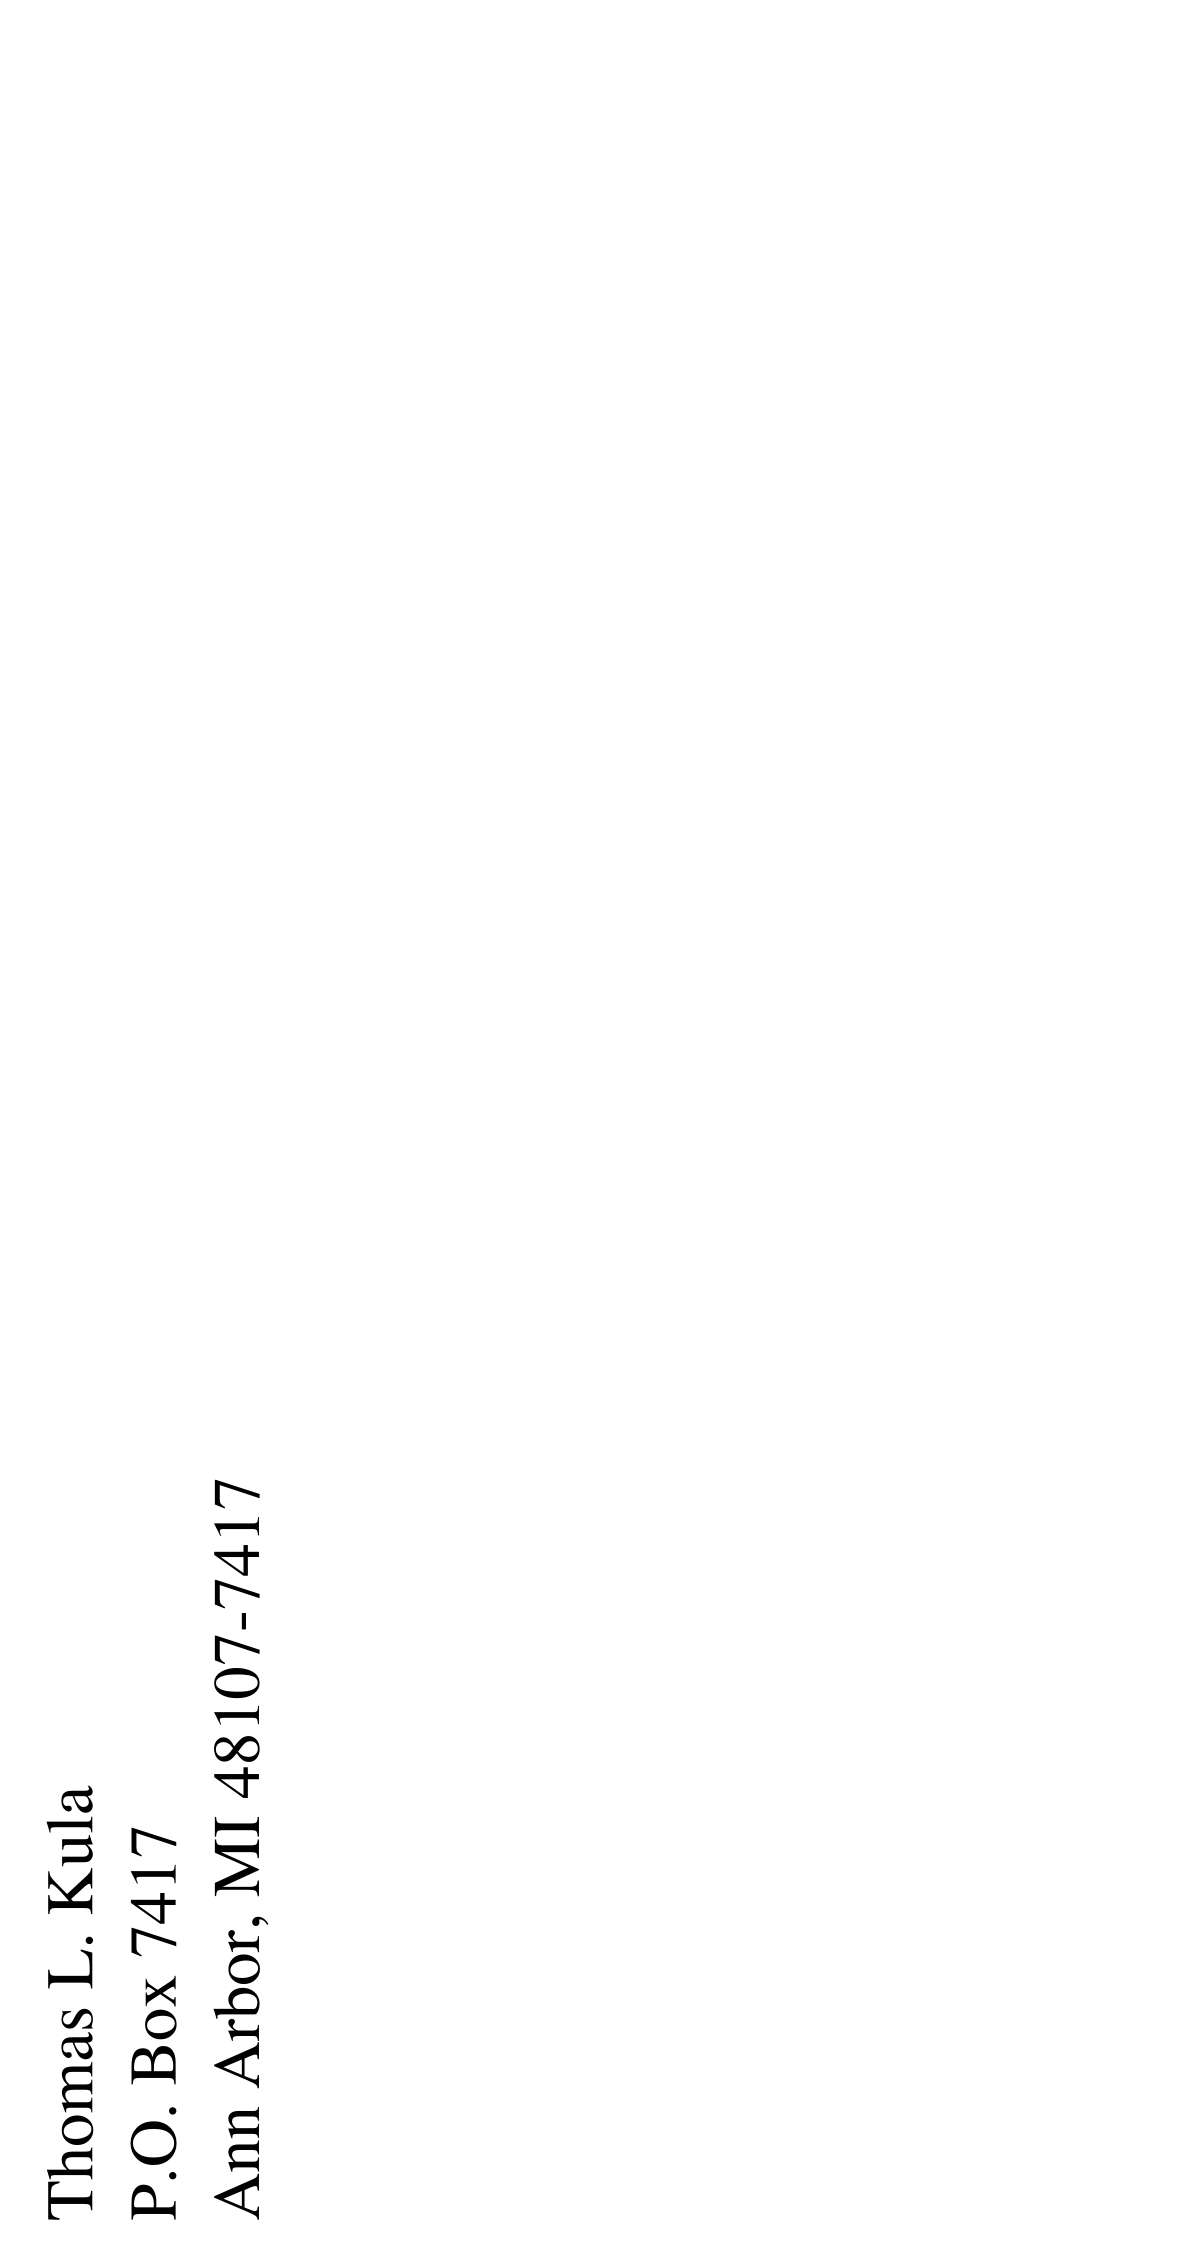
\includegraphics{backpage.png}

\end{document}




